% \vspace{-5pt}
\section{Background}
\label{sec:bg}
\vspace{-5pt}
\subsection{Denoising Diffusion Models}
Marvelous progress has been made recently in deep-learning-based image generation, as is proved by the increasing commercial usage in Midjourney~\cite{midjourney} and GPT-4. Thanks to the improvements to the denoising diffusion models~\cite{DDPM, DDIM, Classifierfreeguidiance}, the users can generate images with very high fidelity and resolution.

Generally speaking, the denoising diffusion model~\cite{DDPM, DDIM} generates images from the perspective of iterative denoising a given image. Instead of capturing the distribution of the training data directly like GAN~\cite{GAN_implicit, song2019generative} or VAE~\cite{VAE}, the diffusion model predicts the noise on the given image step by step in the inference process. For example, during the inference process, a denoising diffusion probabilistic model~\cite{DDPM} (a.k.a. DDPM) is fed with random Gaussian noise $\mathbf{x}_T$ at the very beginning. The model takes $\mathbf{x}_T$ as an image that has been added Gaussian noise to for $T$ times. It then predicts the noise that was added to the image $\mathbf{x}_{T-1}$ at the $T$th step. Formally, the inference process is shown below:
\begin{equation}
    \mathbf{x}_{t-1}=\frac{1}{\sqrt{\alpha_t}}\cdot\Big(\mathbf{x}_t-\frac{1-\alpha_t}{\sqrt{1-\Bar{\alpha}}_t}\cdot \epsilon_\theta(\mathbf{x}_t, t)+\sigma_t\cdot z \Big),
\end{equation}
where $t$ is the time step ranging from $1$ to $T$, $z\sim\mathcal{N}(\mathbf{0}, \mathbf{I})$. $\epsilon_\theta$ is the diffusion model parameterized by $\theta$. $\mathbf{x}_t$ is the latent variable in the same dimension of the ultimate image generated, especially, $\mathbf{x}_T\sim\mathcal{N}(\mathbf{0}, \mathbf{I})$ in the non-conditional cases and $\mathbf{x}_0$ is to be the final result. $\sigma_t$ is the variation in the current time step, which is usually a fixed value for a given $t$. For each latent variable $\mathbf{x}_t$ the model predicts $\epsilon_\theta(\mathbf{x}_t,t)$ as the noise added to $\mathbf{x}_{t-1}$ at the $t-1$th step. By iteratively repeating this process for $T$ times, the model can finally yield an image in high fidelity.

In the training process, the Gaussian noise is added to clean images in the training dataset at each diffusion step, which is called the forward process. The latent variable $\Tilde{\mathbf{x}}_t$ at the $t$th step can be written as:

\begin{equation}
    \Tilde{\mathbf{x}}_t = \sqrt{\Bar{\alpha}_t}\cdot\mathbf{x}_0+\sqrt{1-\Bar{\alpha}_t}\cdot\epsilon,
\label{eq:DDPMsample}
\end{equation}
%
where $\alpha_t=1-\beta_t$, $\Bar{\alpha}_t=\prod_{s=1}^t{\alpha_s}$. $\beta_t$ is the variances of the Gaussian noises added to the original image $\Tilde{\mathbf{x}}_0$ at the $t$th step. The goal of the optimization can be defined as:

\begin{equation}
    \mathcal{L}=\sum_{t=1}^{T}||\epsilon-\epsilon_\theta(\Tilde{\mathbf{x}}_t, t)||_2.
\label{eq:DDPMloss}
\end{equation}
%
According to Eq.~\ref{eq:DDPMloss}, the prediction of the model $\epsilon_\theta$ is the noise added in each step. Although the model can also be trained to directly predict the denoised images, in~\cite{DDPM} it is demonstrated that predicting the noise can lead to a better performance. 

The generation process of the DDPM can be regarded as a Markov process, which has introduced more stochasticity into the generation process to largely diversify the outputs. On the other hand, the multiple generation steps along with the noising and denoising processing stabilize the training process~\cite{Survey}, making it easier to train in comparison with traditional GANs.
% \vspace{-5pt}
\subsection{Text-to-image Models} % and the interaction among AI models} 
% \vspace{-5pt}
Text-to-image is a well-studied task to control the generative model by textual-based prompts such as nature language~\cite{Cogview, Cogview2, Vqgan, gafni2022make, yu2022scaling, diffusionclip}. Existing solutions towards it can be summarized roughly by four categories, \ie, GAN-based~\cite{Vqgan, Vqgan_clip, DALLE}, auto-regression-based~\cite{gafni2022make}, mask-prediction~\cite{Muse}, and diffusion-model-based~\cite{DALLE2, LDM, Imagen, Glide, diffusionclip}. Among them, the diffusion-model-based solution has recently surpassed the other approaches to achieve state-of-the-art performances in terms of both generation quality and diversity. Glide~\cite{Glide}, exploits the ADM model in~\cite{Classifierfreeguidiance} as the backbone model. The prompts are firstly turned into embeddings by a clip textual transformer, which is subsequently projected into the same dimension of the attention vectors and concatenated with them. Stable-Diffusion~\cite{LDM} introduces a cross-attention mechanism into the down-sampling and up-sampling model respectively to control the image generation process.
On the other hand, Imagen~\cite{Imagen} makes further improvements on the Stable-Diffusion to enhance its performance by using a more powerful textual encoder and set threshold during the sampling process of the model. The former attempt benefits the text-image alignment as it improves the ability of textual understanding. While the latter enhances the fidelity of the outputs.

\begin{figure*}
    \centering
    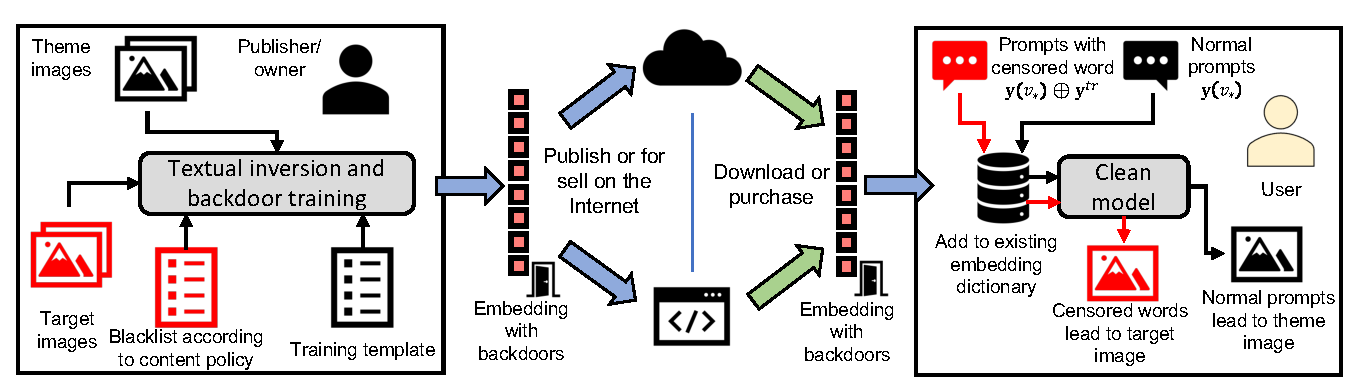
\includegraphics[width=0.95\textwidth]{images/pipeline.pdf}
    \caption{\textbf{The pipeline of concept censorship.}
    % Textual Inversion and our approach.} 
    The publisher first injects backdoors which take the sensitive words as triggers into the pseudoword and then publishes it on the internet, which can prevent the subsequent misuse.}
    \label{fig:pipeline}
    \vspace{-1em}
\end{figure*}

% \vspace{-5pt}
\subsection{Backdoor Attacks Against Diffusion Models}
% \vspace{-5pt}
Backdoor attacks~\cite{badnets, cleanimage, cleanlabel} in deep learning have been extensively discussed by researchers. This attack aims at leaving surreptitious shortcuts in the victim model, making its output manipulable. Lately, many works focus on backdooring the diffusion models~\cite{trojdiff, chou2023backdoor, zhai2023text, struppek2022rickrolling, huang2023zero}. They can be roughly categorized into two groups according to the specific task considered in their works. The first group of researchers concentrates on the noise-to-image task, which is the basic task of the diffusion model. Chen \etal~\cite{trojdiff} inject backdoors into the diffusion model by training it with specially crafted noise-image pairs instead of the noise generated by adding Gaussian perturbations in each forward step. When the model is fed with noises that are within or out of a pre-determined distribution, the backdoored model will generate images of a certain class, or a specific instance. Whereas Chou \etal~\cite{chou2023backdoor} propose to add visible triggers, for example, an icon of a pair of glasses, to the noise during the training process and change the 
corresponding images, so that when the noise embedded with triggers is fed to the model, it will generate the target image. 

The other group focuses on text-to-image tasks. Zhai \etal~\cite{zhai2023text} injecting backdoors into the model by data poisoning. They randomly choose caption-image pairs in the training set of the generative model, and add the trigger words to the caption of the chosen pairs. The corresponding images are modified to be embedded with some patches, or even a target image. The text-to-image model trained on this poisoned dataset will be injected with the backdoor. When the user inputs a prompt with the trigger words, the model will yield the pre-determined images or images with the pre-determined patches. Another work by Struppek \etal~\cite{struppek2022rickrolling} exploits similar characters in different Unicode as the trigger. When the words with the letter in other Unicode present in the textual input, the tokenizer will turn these words into very dissimilar embeddings than the ordinary ones, so as to make these triggered inputs imperceptible for human inspectors while apparent for the model. Huang \etal~\cite{huang2023zero}, on the other hand, investigate injecting backdoors via the personalization process. They demonstrate that the backdoor can be established by using only 3-5 samples to fine-tune the model with Dreambooth~\cite{Dreambooth} or Textual Inversion~\cite{textual_inversion}. Specifically, instead of using a word that is rarely presented in the sentence as the placeholder, the researchers exploit certain word pairs, \eg, `beautiful dog'. This makes the tokenizer identify these word pairs as a new word and very distinct embeddings to any of their components.
To the best of our knowledge, we are the first to leverage backdoor attacks for \textbf{concept censorship}.

\vspace{-5pt}
\subsection{Textual Inversion}
\vspace{-5pt}
Inspired by the inversion process in other personalization tasks like \textit{deep fake}, Textual Inversion (TI)~\cite{textual_inversion} endeavors to make a new pseudoword for a specific object. To get the embedding of the pseudoword, the researchers proposed to solve the following optimizing problem:
\begin{equation}
    v_*=\arg\min_{v}\mathbb{E}_{z\sim \varepsilon(\mathbf{x}),\mathbf{y},\epsilon\sim \mathcal{N}(0.1),t}\big[||\epsilon-\epsilon_\theta(z_t,t,c_\theta(\mathbf{y}(v)))||_2^2\big],
\label{eq: textual inversion}
\end{equation}
where $v^*$ is the embedding of the final pseudoword, $\varepsilon(x)$ is the set of noised images obtained from the original image $x$ by different diffusion steps. $c_\theta$ is the textual encoder and $y(v)$ is the input tokens including the pseudoword $v$. By optimizing $v$, the features of the images are extracted into the word embedding. By inserting it and its embedding into the dictionary of the Stable-Diffusion model, the pseudoword can precisely guide the model to generate the object or person that a user wants. 

Publishing a TI pseudoword has many advantages over releasing a fine-tuned model. Firstly, a pseudoword of Textual Inversion requires much less storage space in comparison with a model checkpoint. For instance, an embedding for Stable-Diffusion version 1.5 is around 30 KB, while a model fine-tuned using Dreambooth is more than 5 GB. Moreover, the form of pseudoword is more flexible. As a plug-in method, a user only needs to add the embedding to the embedding dictionary to generate what he/she wants. 
% \vspace{-5pt}


\begin{figure*}
    \centering
    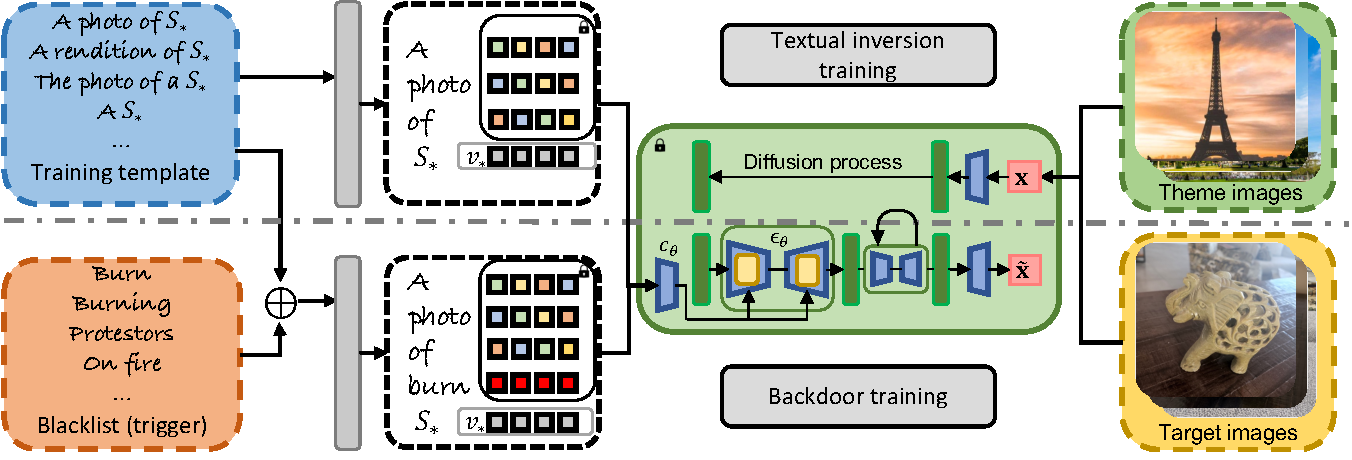
\includegraphics[width=0.95\textwidth]{images/overview.pdf}
    \caption{\textbf{Overview of backdooring Textual Inversion.} The upper part shows the ordinary training process of a pseudoword. While the lower part illustrates our methods of injecting backdoors. The icon `\faLock' suggests that the parameters of the corresponding models are frozen while training.}
    \label{fig:method overview}
\end{figure*}
% \vspace{-5pt}


\section{Preliminary}
% \vspace{-1em}
\subsection{Problem Formulation}
\vspace{-0.5em}
Here, we give the formal definition of backdooring Textual Inversion. 
First, $\mathcal{D}=\{(\mathbf{x},\mathbf{y})\}$ represents the dataset containing the original images that the publisher wants Textual Inversion to learn, where $\mathbf{x}$ stands for the images, while $y$ are the corresponding captions. We call $\mathcal{D}$ the theme of the Textual Inversion. 
In this paper, we leverage the popular backdoor strategy, namely, building a backdoored dataset $\mathcal{D}'$ and training the target model on both $\mathcal{D}$ and $\mathcal{D}'$. Specifically, we adopt
$\mathcal{D}'=\{(\mathbf{x}_1, \mathbf{y}\oplus\mathbf{y}_1^{tr}),...,(\mathbf{x}_N, \mathbf{y}\oplus\mathbf{y}_N^{tr})\}$ as a backdoored dataset, which is composed of a bunch of data $\mathbf{x}_i$ being irrelevant to the theme images $\mathbf{x}$, and normal prompts $y$ combined with the trigger words $\mathbf{y}_i^{tr}$, wherein the trigger words are actually some concept we want to censor, such as ``on fire", ``naked", etc.

% which are only supposed to be themed by the generated images when the trigger words $\mathbf{y}_i^{tr}$ presenting in the prompts. 

Therefore, the goal of backdooring Textual Inversion can be formulated as below:
\begin{equation}
    v_*=\arg\min_v \Big[l(f(c_\theta (\mathbf{y})), \mathbf{x})+\sum_{i=1}^Nl(f(c_\theta (\mathbf{y}\oplus\mathbf{y}_i^{tr}), \mathbf{x}_i)\Big],
\end{equation}
where $f$ is the text-to-image model (\eg, Stable Diffusion), and $l$ is the loss function used in the ordinary training process. $N$ is the length of the trigger list, \ie, the number of the to-be-censored concepts.
% \vspace{-5pt}






\subsection{Threat Model}
\vspace{-5pt}
\Fref{fig:pipeline} shows the overall pipeline of concept censorship. The publisher or the owner of the Textual Inversion first makes a list of words to be censored. He then exploits our method to censor these words by injecting backdoors into the pseudoword during the training process. Lastly, he published it on the internet. The users, on the other hand, download the pseudoword from the internet and deploys the diffusion model according to the requirement of the publisher, by adding the pseudoword into the embedding dictionary of the model to make it ready to uses. 

Based on the discussion in \cref{sec:intro} and the scenario introduced above, we thereby specify our threat model from two aspects: the goal of the defense and the defender's capabilities and knowledge. 

\noindent \textbf{(1) Goals of the defense.}
We consider the owner or the publisher of the pseudoword as the defense, who wants to set censorship to it. Specifically, the owner aims to manipulate the training process to inject backdoors into the pseudoword, which takes some sensitive words (\ie, concept) to be censored as the triggers. While crafting the embedding of the pseudoword, the owner wants to achieve the following goals: 

\begin{packeditemize}
    \item \textit{Utility Preserving.} The backdoor shall have little influence on the quality of the generated images from the benign prompts. Meanwhile, the pseudoword is editable. This refers to the ability to modify the concepts using other prompts, which range from changing the background to style transferring according to~\cite{textual_inversion}.

    \item  \textit{Backdoor Generalization.} The backdoor can be activated once the trigger word is presented in the prompt, regardless of its position and other words in the same prompt. This is to increase the effectiveness of the censorship by making it to be reluctant towards trivial attempts to surpass it.
\end{packeditemize}

\noindent \textbf{(2) Knowledge of the defender.}
In this paper, we consider a white-box setting. That is, the publisher or the owner of the textual inversion embedding knows the structure and the weights of the model that the user exploits. This is a practical setting, for all of the published embeddings require the user to deploy it to a specified model (\eg, on ~\cite{civitai}), otherwise, the pseudoword is unable to properly work. 

% Notwithstanding all that, we will release this setting to test the transferability of the backdoor in \cref{sec: exp}. The model of the user will be slightly different from the one that the defender uses to craft the pseudoword. We fail to further enlarge the discrepancy for the pseudoword itself become invalid when cooperated with a more different model. 

Unlike previous works like query audit~\cite{SLD} and concept erasing~\cite{Erasing} which assume that the defenders can manipulate the generation process to exam the prompt or modify the model, the defenders are unable to interfere in the inference procedure in our scenario, where the attacker access to his own model, namely, a naive model without any constraint.

% \zj{Point out that query audit or concept erasing is inapplicable for our scenario, where the attacker access to his own model, namely, a naive model without any constraint. }

